%Version 3.1 December 2024
%
% International Journal of Data Science and Analytics (IJDSA)
% Springer Nature ? sn-jnl class, two-column format [iicol]
%
% Compile sequence: pdflatex -> bibtex -> pdflatex -> pdflatex
%

\documentclass[pdflatex,sn-mathphys-num,iicol]{sn-jnl}

%%%% Standard Packages
\usepackage{graphicx}
\usepackage{multirow}
\usepackage{amsmath,amssymb,amsfonts}
\usepackage{amsthm}
\usepackage{mathrsfs}
\usepackage[title]{appendix}
\usepackage{xcolor}
\usepackage{textcomp}
\usepackage{manyfoot}
\usepackage{booktabs}
\usepackage{tabularx}
\usepackage{longtable}
\usepackage{array}
\usepackage{siunitx}
\usepackage{subcaption}
\usepackage{float}
\usepackage{microtype}
\setlength{\emergencystretch}{3em}

\newcolumntype{P}[1]{>{\centering\arraybackslash}p{#1}}

\raggedbottom

\begin{document}
	
	%%---------------------------------------------------------
	%%  TITLE
	%%---------------------------------------------------------
	\title[Science in the Colombian Public Sphere]{Science in the Colombian Public Sphere: A Digital Humanities and NLP Analysis of Opinion Columns (2018--2020)}
	
	%%---------------------------------------------------------
	%%  AUTHORS AND AFFILIATIONS
	%%---------------------------------------------------------
	\author*[1]{\fnm{Karen Melissa} \sur{Gomez-Montoya}}\email{kmgomezm@eafit.edu.co}
	
	\author[1]{\fnm{Biviana Marcela} \sur{Su{\'a}rez-Sierra}}\email{bmsuarezs@eafit.edu.co}
	
	\affil*[1]{\orgname{Universidad EAFIT}, \orgaddress{\city{Medell{\'i}n}, \country{Colombia}}}
	
	%%---------------------------------------------------------
	%%  ABSTRACT  (150?250 words per IJDSA guidelines)
	%%---------------------------------------------------------
	\abstract{%
		This article examines how science is discursively represented in Colombian opinion journalism through a computational analysis of approximately 13,000 opinion columns published between 2018 and 2020 in three major national newspapers. Using natural language processing techniques---including semantic search with text embeddings, named entity recognition, topic modeling, and part-of-speech tagging---we identify textual fragments containing references to science, grounded in the UNESCO Thesaurus as a conceptual framework. Results show that 30.4\% of columns contain at least one science-related mention, concentrated primarily in Science and Research Management and Pollution, Disasters and Safety. Scientific discourse peaks notably in March--April 2020, coinciding with the beginning of the COVID-19 pandemic. Science appears predominantly associated with governmental actors, international organizations, and environmental concerns, framed as an instrumental resource for crisis management and public policy rather than as abstract disciplinary knowledge. These findings contribute to understanding the social appropriation of science in Latin American media contexts.%
	}
	
	%%---------------------------------------------------------
	%%  KEYWORDS  (4?6 per IJDSA guidelines)
	%%---------------------------------------------------------
	\keywords{Digital humanities, Discourse analysis, Natural language processing, Public opinion, Colombia}
	
	\maketitle
	
	%%---------------------------------------------------------
	%%  SECTION 1 ? INTRODUCTION
	%%---------------------------------------------------------
	\section{Introduction}\label{sec:intro}
	
	Science occupies a central position in contemporary public debates. Decisions related to health, the environment, the economy, or education rely on scientific and technological knowledge with the aim of promoting collective well-being and addressing complex problems that affect humanity, such as the development and distribution of vaccines (\cite{Chakravartty2022}). In this context, the ways in which science, scientists, and scientific organizations are mentioned, represented, and perceived in media discourse play a key role in shaping public opinion and in legitimizing policies and collective actions (\cite{Mede2022}).
	
	Discussions about science in the public sphere have frequently focused on the level of societal trust in science and in scientists (\cite{Cologna2025, Sturgis2021, Mede2022}), as well as on issues related to science communication, outreach, and dissemination. To a lesser extent, research has examined the broader perceptions that different communities hold about science, typically through public opinion surveys.
	
	In Latin America, and particularly in Colombia, these perceptions have been studied primarily through national surveys. In the Colombian case, three such measurements have been conducted: the first in 1994, followed by one in 2004 and another in 2012, the latter administered by the Observatorio Colombiano de Ciencia y Tecnolog{\'i}a (\cite{Daza_Caicedo2014}). For the organizations that constitute the Science, Technology, and Innovation (STI) ecosystem, both at the national and regional levels, monitoring these public perceptions is essential. Understanding what Colombians think about science makes it possible to improve processes of social appropriation of knowledge, guide political and academic agendas, evaluate communication strategies, and identify the social imaginaries circulating in the public sphere around scientific activity (\cite{Daza_Caicedo2014}).
	
	However, beyond surveys, the media represent a privileged arena for observing how science is discursively articulated in the public sphere. Opinion columns, in particular, have been shown to possess the capacity to influence and reshape readers’ perceptions and attitudes, both among elites and the general public (\cite{Coppock2018}). At times, scientists themselves turn to this format to intervene in public debate. Nevertheless, previous studies suggest that when writing opinion columns, scientists often lack sufficient rhetorical resources to persuade readers holding divergent positions, tending instead to address audiences who already share similar views (\cite{Syfert2025}).
	
	Opinion columns frequently address issues of high scientific and social relevance, such as vaccines, the environment, or climate change. In the Colombian context, this genre has been characterized by a strong argumentative and persuasive orientation, as well as by its focus on current affairs, where the primary objective is to convince the reader (\cite{CaroLopera2020}). Despite this, little is still known about how science is discursively integrated into this type of text and with which actors, organizations, topics, and events it is associated.


	Against this backdrop, the present study analyzes a sample of approximately 13,000 opinion columns published in three widely circulated Colombian print media outlets, in order to address the following research question: with which topics, organizations, actors, and events is science associated in opinion discourse in Colombia, and what discursive patterns emerge from these associations? To this end, the article proposes a strategy grounded in natural language processing techniques that enables the identification of explicit references to science within the corpus and the examination of their co-occurrences with entities, actors, and domain-specific vocabulary. The aim is to better understand how science is constructed and represented within the Colombian public sphere.
	
	%%---------------------------------------------------------
	%%  SECTION 2 ? METHODOLOGY
	%%---------------------------------------------------------
	\section{Methodology}\label{sec:methodology}
	
	To address the proposed research question, text mining and natural language processing (NLP) methods were employed. The methodology was structured into three main stages. First, references to science were identified within the opinion columns in order to construct a subcorpus. Second, algorithms were applied to analyze authorship, actors, topics, and vocabulary in both the subcorpus and the full corpus, enabling comparative analysis. Finally, the extracted elements were interpreted in light of national events occurring during the publication periods of the opinion columns, and the affiliations of both authors and referenced actors were identified to enrich the analysis. The overall procedure is summarized in the flowchart presented in Figure \ref{fig:diagramaflujo} and is described in detail in the following section. All analyses were conducted using Python 3.12.7 \cite{python2023}.\footnote{Available at \url{https://www.python.org/downloads}}. 
	
	\begin{figure}[t]
		\centering
		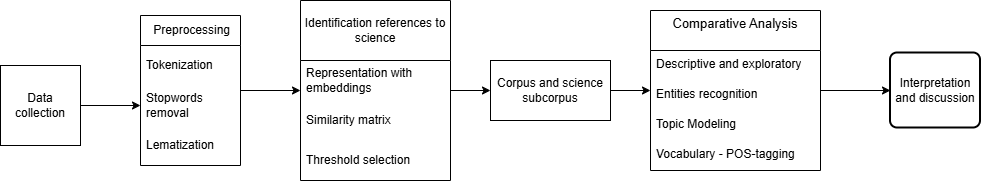
\includegraphics[width=\columnwidth]{figures/diagrama_paper_ciencia.png}
		\caption{Flowchart of the applied methodology.}
		\label{fig:diagramaflujo}
	\end{figure}
	
	\subsection{Data Collection}\label{subsec:data}
	
	A total of 13,000 opinion columns were collected from three widely circulated Colombian print media outlets. These columns were published between January 2018 and December 2020. At this stage, the only selection criterion was that the column consist entirely of written text and not require video or audio to understand its content. The columns were not selected based on any specific topic. For each opinion column, the following metadata were collected: the name of the newspaper, the author, the date, the title, the full text (body) of the column, and the URL. Each text was verified to ensure uniqueness (i.e., no duplicated columns), and author names were standardized. After this process, a unique identification number was assigned to each opinion column.
	
	\begin{table}[t]
		\caption{Distribution of columns and authors by newspaper.}
		\label{tab:col_autores_periodico}
		\begin{tabular}{@{}lccc@{}}
			\toprule
			\textbf{Newspaper} & \textbf{Columns} & \textbf{Authors} & \textbf{\% Total} \\
			\midrule
			El Espectador & 10509 & 263 & 76.84 \\
			El Tiempo     & 1982  & 249 & 14.49 \\
			Semana        & 1185  & 96  & 8.66  \\
			\botrule
		\end{tabular}
	\end{table}
	
	
	\subsection{Preprocessing}\label{subsec:preprocessing}
	
	When working with large volumes of text, as in the case of this corpus of opinion columns, analysis cannot begin directly with the raw material. It is first necessary to transform the data into a format that can be interpreted by NLP algorithms \cite{Chai2022}. This preparatory stage, known as preprocessing, involves a series of methodological decisions aimed at cleaning, structuring, and standardizing the text prior to modeling. In this study, the procedure began with an initial cleaning of each column, during which URLs, hashtags, and social media user mentions (@) were removed, along with redundant whitespace and characters other than letters, numbers, and standard punctuation marks. This cleaning stage reduced noise and helped homogenize the corpus.
	
	Once cleaned, the text was segmented into basic analytical units through tokenization. This step consists of dividing the text into smaller fragments (tokens), which in this case correspond to individual words \cite{Tyagi_text}. Thus, a sentence such as ``Tokenization is fundamental'' is transformed into the sequence ``Tokenization,'' ``is,'' and ``fundamental.'' Although seemingly straightforward, this operation is essential because it converts unstructured text into a computationally manageable structure, enabling the calculation of frequencies, co-occurrences, and other linguistic metrics.
	
	Subsequently, and depending on the specific requirements of each algorithm applied, so-called stopwords were removed. These are highly frequent words that serve grammatical functions (such as articles, prepositions, pronouns, or conjunctions) and, while essential for syntactic coherence, typically contribute little semantic information in tasks such as topic modeling \cite{Siino2024}. In addition to improving the interpretability of the models, their removal reduces the dimensionality of the corpus, which is computationally advantageous. Because stopword lists are language- and context-dependent, the lists used in this study were reviewed and adjusted prior to application, particularly in the stage preceding topic modeling.
	
	Finally, the process included lemmatization, that is, the reduction of words to their canonical or base form \cite{Orellana2018}. This standardization makes it possible to group morphological variants under a single lexical entry—for example, converting conjugated verbs to the infinitive or transforming plural nouns into the singular—which is crucial for frequency analyses and lexical studies. The selection of the lemmatization model required particular attention. In an initial stage, the lemmatizer from the spaCy library in Python was used; however, limitations in accuracy for Spanish were observed. For this reason, the Stanford Stanza library model \cite{qi2020stanza}, based on neural networks, was ultimately adopted, as it provided greater accuracy in lemma identification. Lemmatization was applied prior to lexical analysis and part-of-speech (POS) tagging.\\

	
	\subsection{Identification of References to Science}\label{subsec:identification}
	
	To advance the objective of this study---namely, to understand how science is represented in opinion discourse in Colombia---it was necessary to systematically identify references associated with the scientific field within the previously described corpus. To this end, a strategy based on semantic search was designed. Semantic search is an information retrieval method that enables the identification of meaning-based relationships beyond the literal matching of keywords \cite{Wei2022}. Unlike traditional lexical search, this approach retrieves texts according to their conceptual proximity, incorporating phenomena such as synonymy, terminological variation, and semantic affinity among expressions.
	
	The strategy consisted of representing both the corpus of approximately 13,000 columns and the 17 UNESCO Thesaurus categories for Science through embeddings (vector representations that capture the contextual meaning of texts). Each Thesaurus category (conceived as a semantic field grouping representative terms from different scientific areas) was encoded as a semantic query, composed of the set of words and expressions associated with that category. In parallel, the corpus fragments were transformed into comparable vector representations.
	
	
	Once these vectors were obtained, semantic similarity between each corpus fragment and each of the 17 categories was calculated using cosine similarity---a metric that quantifies the degree of proximity between two vectors in semantic space. This procedure made it possible to estimate, for each text fragment, a set of affinity scores with respect to the different Thesaurus categories. Based on these scores, a similarity ranking was generated, and each fragment was assigned to the category with the highest recorded value.
	
	
	\subsubsection{Definition of Science: UNESCO Thesaurus}\label{subsubsec:thesaurus}
	
	The words used to represent science were those included in the UNESCO Thesaurus. The UNESCO Thesaurus ``is a controlled and structured list of terms for subject analysis and the retrieval of documents and publications in the fields of education, culture, natural sciences, social and human sciences, communication, and information'' \cite{unesco_thesaurus_1977}. Its first English version was published in 1977, and it is periodically revised and updated. For the purposes of this study, the list specifically labeled Science, specialized in the natural sciences, was used. The Spanish-language version of this list was employed for the analysis. This list made it possible to approach science through the words that compose it or are used to identify it across different areas. The category comprises 17 subcategories, each containing between 24 and 84 terms. For reference, a table including the first terms of each category is presented in Table~\ref{tab:categorias_ciencia}.
	

\begin{table*}[t]
	\centering
	\footnotesize
	\caption{UNESCO Thesaurus Science Categories and the First Terms of Each.}
	\label{tab:categorias_ciencia}
	
	\begin{tabular}{@{}p{3.5cm}p{2cm}p{8.5cm}@{}}
		\toprule
		\textbf{Subcategory} & \textbf{No. of terms} & \textbf{First 10 terms} \\
		\midrule
		
		Scientific approach & 50 & Accessibility, Basic sciences, Benchmarking, Calibration, Case studies, Causal analysis, Cause and effect, Comparative analysis, Cross national analysis, Design \\
		
		Science and research management & 62 & Academies of science, Applied research, Appropriate technology, Automation, Choice of technology, Diffusion of technology, Digital divide, Digital transformation, Economics of science, Engineers \\
		
		Mathematics and statistics & 34 & Algebra, Algorithms, Arithmetic, Calculus, Combinatorial mathematics, Correlation, Data visualization, Equations, Extrapolation, Factor analysis \\
		
		Physical sciences & 56 & Acoustics, Aerodynamics, Atomic structure, Cooling, Cosmic radiation, Crystallography, Diffusion, Electrical properties, Electricity, Electromagnetic waves \\
		
		Chemical sciences & 50 & Acids, Biochemical analysis, Carbon, Carbon dioxide, Chemical analysis, Chemical compounds, Chemical effects, Chemical elements, Chemical kinetics, Chemical processes \\
		
		Space sciences & 24 & Astronomical systems, Astronomy, Astrophysics, Black holes, Celestial mechanics, Cosmic matter, Cosmology, Earth (planet), Galaxies, Gravitation \\
		
		Earth sciences & 61 & Biogeochemistry, Carbonate rocks, Coastal erosion, Continental drift, Desert soils, Earth sciences, Earth's crust, Erosion, Fossils, Gems \\
		
		Geography and oceanography & 84 & Adriatic Sea, Aegean Sea, Antarctic Ocean, Aral Sea, Arctic Ocean, Atlantic Ocean, Baltic Sea, Basins, Bathymetric charts, Bathymetry \\
		
		Meteorology & 34 & Agroclimatology, Antarctic regions, Arctic regions, Arid zones, Atmosphere, Atmospheric circulation, Atmospheric pressure, Bioclimatology, Climate, Climatic data \\
		
		Hydrology & 46 & Aquifers, Brackish water, Drainage, Drainage basins, Drinking water, Ecohydrology, Freshwater, Groundwater, Hydrogeological maps, Hydrogeology \\
		
		Environmental sciences and engineering & 52 & Animal rights, Aquatic environment, Biological control, Botanical gardens, Desalination, Ecological research, Ecology, Energy balance, Energy conservation, Energy consumption \\
		
		Pollution, disasters and safety & 54 & Accident prevention, Accidents, Acid rain, Agricultural wastes, Air pollution, Avalanches, Climate change, Climate change adaptation, Damage, Dangerous materials \\
		
		Natural resources & 53 & Animal behaviour, Animal ecology, Animal migration, Animal resources, Aquatic ecosystems, Biodiversity, Biogas, Biological adaptation, Biomass, Biomass energy \\
		
		Biology & 75 & Ageing, Anatomy, Artificial procreation, Bacteria, Bacteriology, Biochemicals, Biochemistry, Bioethics, Biogenesis, Biological effects \\
		
		Natural sciences & 50 & Algae, Animal diseases, Animal genetics, Animal nutrition, Animal taxonomy, Animals, Anthropology, Aquatic animals, Aquatic plants, Birds \\
		
		Medical sciences & 54 & Acupuncture, Aerospace medicine, Brain research, Clinical medicine, Dentistry, Dietetics, Disease control, Drug control, Drug policy, Drugs \\
		
		Pathology & 40 & AIDS, Albinism, Blindness, Cancer, Cardiovascular diseases, Clinical psychology, Colour blindness, Deaf dumbness, Deafness, Disabilities \\
		
		\bottomrule
	\end{tabular}
\end{table*}

\normalsize


	
	\subsubsection{Embedding Model Selection}\label{subsubsec:embedding}
	
	For this study, a pre-trained embeddings model was selected. This means that the model had been previously developed and trained on large volumes of textual data, enabling it to capture complex semantic relationships without requiring retraining from scratch. This strategy is grounded in the framework of transfer learning, whereby a model trained on a general task can be effectively reused in different contexts~\cite{Hosna2022}. In this way, the corpus of opinion columns could be analyzed by leveraging previously acquired linguistic knowledge, thereby reducing computational costs and development time.
	
	
	The selection of the embeddings model required consideration of several key criteria. First, the model needed to be optimized for semantic similarity tasks, since the central objective was to measure the conceptual proximity between corpus fragments and the UNESCO Thesaurus categories for Science. Second, it had to provide robust support for the Spanish language, given that the analyzed corpus consists of opinion columns published in Colombia. Finally, the model's size—understood in terms of the number of parameters and memory requirements— was evaluated, ensuring that it did not exceed 500 million parameters in order to maintain computational feasibility.

	
	The final decision was informed by the results of the Massive Multilingual Text Embedding Benchmark (MMTEB), a large-scale comparative evaluation of multilingual embedding models~\cite{enevoldsen2025mmtebmassivemultilingualtext}. This benchmark enables the comparison of model performance across tasks such as information retrieval and semantic similarity. Among the evaluated models, one that achieved a strong balance between performance in Spanish, effectiveness in similarity tasks, and moderate size was \texttt{embeddinggemma-300m}, developed by Google~\cite{vera2025embeddinggemmapowerfullightweighttext}. This model comprises approximately 300 million parameters and supports a context window of up to 2048 tokens, making it suitable for processing relatively long text fragments without losing semantic coherence.
	
	Once the model was selected, the corpus was prepared for vector encoding. Because opinion columns often address multiple topics within a single text, working with complete documents would hinder the precise identification of references to science. For this reason, each column was divided into fragments (chunks) of approximately 150 words, with a minimum length of 100 words and an overlap of 20 words between consecutive fragments. Establishing a minimum length is important because the segmentation is performed sequentially from the beginning of the text, which may result in a final fragment that is excessively short; when this occurred, the fragment was merged with the preceding one. The overlap between fragments helps preserve contextual continuity and prevents abrupt semantic breaks. Additionally, this procedure ensures that each fragment remains within the model’s maximum token limit.
	
	Subsequently, a representative embedding was computed for each fragment of the corpus. In a parallel manner, for each UNESCO Thesaurus subcategory, a text was constructed by concatenating its corresponding keywords, and an embedding was generated from this combined string. In this way, both the column fragments and the Thesaurus categories were represented within the same vector space.
	
	\subsubsection{Cosine Similarity}\label{subsubsec:cosine}
	
	Once both the corpus fragments and the UNESCO Thesaurus subcategories had been represented within the same vector space through embeddings, it was necessary to define a metric to quantify their semantic proximity. The measure used to evaluate similarity between the encoded texts was cosine similarity, one of the most widely employed metrics in information retrieval and natural language processing~\cite{jurafsky2025}.
	
	In this context, let $\mathbf{u}$ denote the vector corresponding to a fragment (chunk) of an opinion column, and let $\mathbf{v}$ represent the vector associated with one of the 17 UNESCO Thesaurus categories for Science. The cosine similarity between these two vectors is defined as:
	
	\begin{equation}
		\text{sim}_{\cos}(\mathbf{u}, \mathbf{v}) =
		\frac{\mathbf{u} \cdot \mathbf{v}}
		{\lVert \mathbf{u} \rVert \, \lVert \mathbf{v} \rVert}
		\label{eq:cosine}
	\end{equation}
	
	
	where $\mathbf{u} \cdot \mathbf{v}$ denotes the dot product between the vectors, and $\lVert \mathbf{u} \rVert$ and $\lVert \mathbf{v} \rVert$ correspond to their Euclidean norms. This expression computes the cosine of the angle formed by the two vectors in semantic space.
	
	The value of this measure ranges between $-1$ and $1$. A value close to $1$ indicates that the vectors point in the same direction (an angle close to $0$ degrees), implying high semantic similarity. A value close to $0$ indicates orthogonality (an angle close to $90$ degrees), that is, the absence of a meaningful semantic relationship. A value close to $-1$ corresponds to vectors pointing in opposite directions (an angle close to $180$ degrees), which in semantic terms would imply opposition or extreme dissimilarity. In practice, when working with embeddings generated by modern language models, values tend to concentrate in the $[0,1]$ range due to the nature of these representations.
	
	In the procedure implemented in this study, for each corpus fragment $\mathbf{u}$, cosine similarity was computed with each of the 17 vectors $\mathbf{v}$ corresponding to the Thesaurus categories. This yielded, for every fragment, a set of 17 semantic affinity scores. The category assigned to a given fragment was the one with the highest similarity value. In this way, each chunk of the opinion columns was classified according to the scientific field with which it exhibits the greatest conceptual proximity.
	 
	
	\subsubsection{Selection Threshold}\label{subsubsec:threshold}
	
	Once the full corpus of opinion columns had been segmented, a total of $m = 62{,}651$ fragments were obtained. Each fragment was represented by an embedding and compared with the $n = 17$ vectors corresponding to the UNESCO Thesaurus categories for Science. For each pair $(i,j)$, cosine similarity was computed between the embedding of text fragment $i$ and the embedding of category $j$. This procedure yielded a similarity matrix $\mathbf{S} \in \mathbb{R}^{m \times n}$, defined as:
	
	\begin{equation}
		\mathbf{S} =
		\begin{bmatrix}
			s_{1,1} & s_{1,2} & \cdots & s_{1,n} \\
			s_{2,1} & s_{2,2} & \cdots & s_{2,n} \\
			\vdots  & \vdots  & \ddots & \vdots  \\
			s_{m,1} & s_{m,2} & \cdots & s_{m,n}
		\end{bmatrix}
		\label{eq:matrix}
	\end{equation}
	
	where each element $s_{i,j} = \text{sim}_{\cos}(\text{text}_i, \text{category}_j)$ represents the degree of semantic proximity between fragment $i$ and category $j$.
	
	From this matrix, for each fragment $i$, the category with the highest similarity value was identified:
	\[
	j^*(i) = \arg\max_{j \in \{1,\dots,17\}} s_{i,j}.
	\]
	
	However, this assignment criterion implies that every fragment is classified into some category, even when its similarity levels are low in absolute terms. For this reason, a selection threshold $\tau \in [0,1]$ was introduced. A fragment $i$ is considered an effective mention of science only if
	\[
	\max_{j} s_{i,j} \geq \tau.
	\]
	
	To determine an appropriate value for $\tau$, a manual validation was conducted based on close reading of a sample of fragments. Values below $0.4$ tended to correspond to weak semantic associations. From fragments whose maximum similarity score exceeded $0.4$, ten fragments were randomly selected for each of the 17 Thesaurus categories, yielding a validation sample of 170 fragments. Each fragment was manually classified as either an ``effective mention of science'' or a ``non-mention.''
	
	Figure~\ref{fig:accuracy-umbral} shows the evolution of accuracy as a function of the threshold $\tau$. Each point on the curve corresponds to the accuracy obtained by applying a specific value of $\tau$ to the validation sample.
	
	\begin{figure}[t]
		\centering
		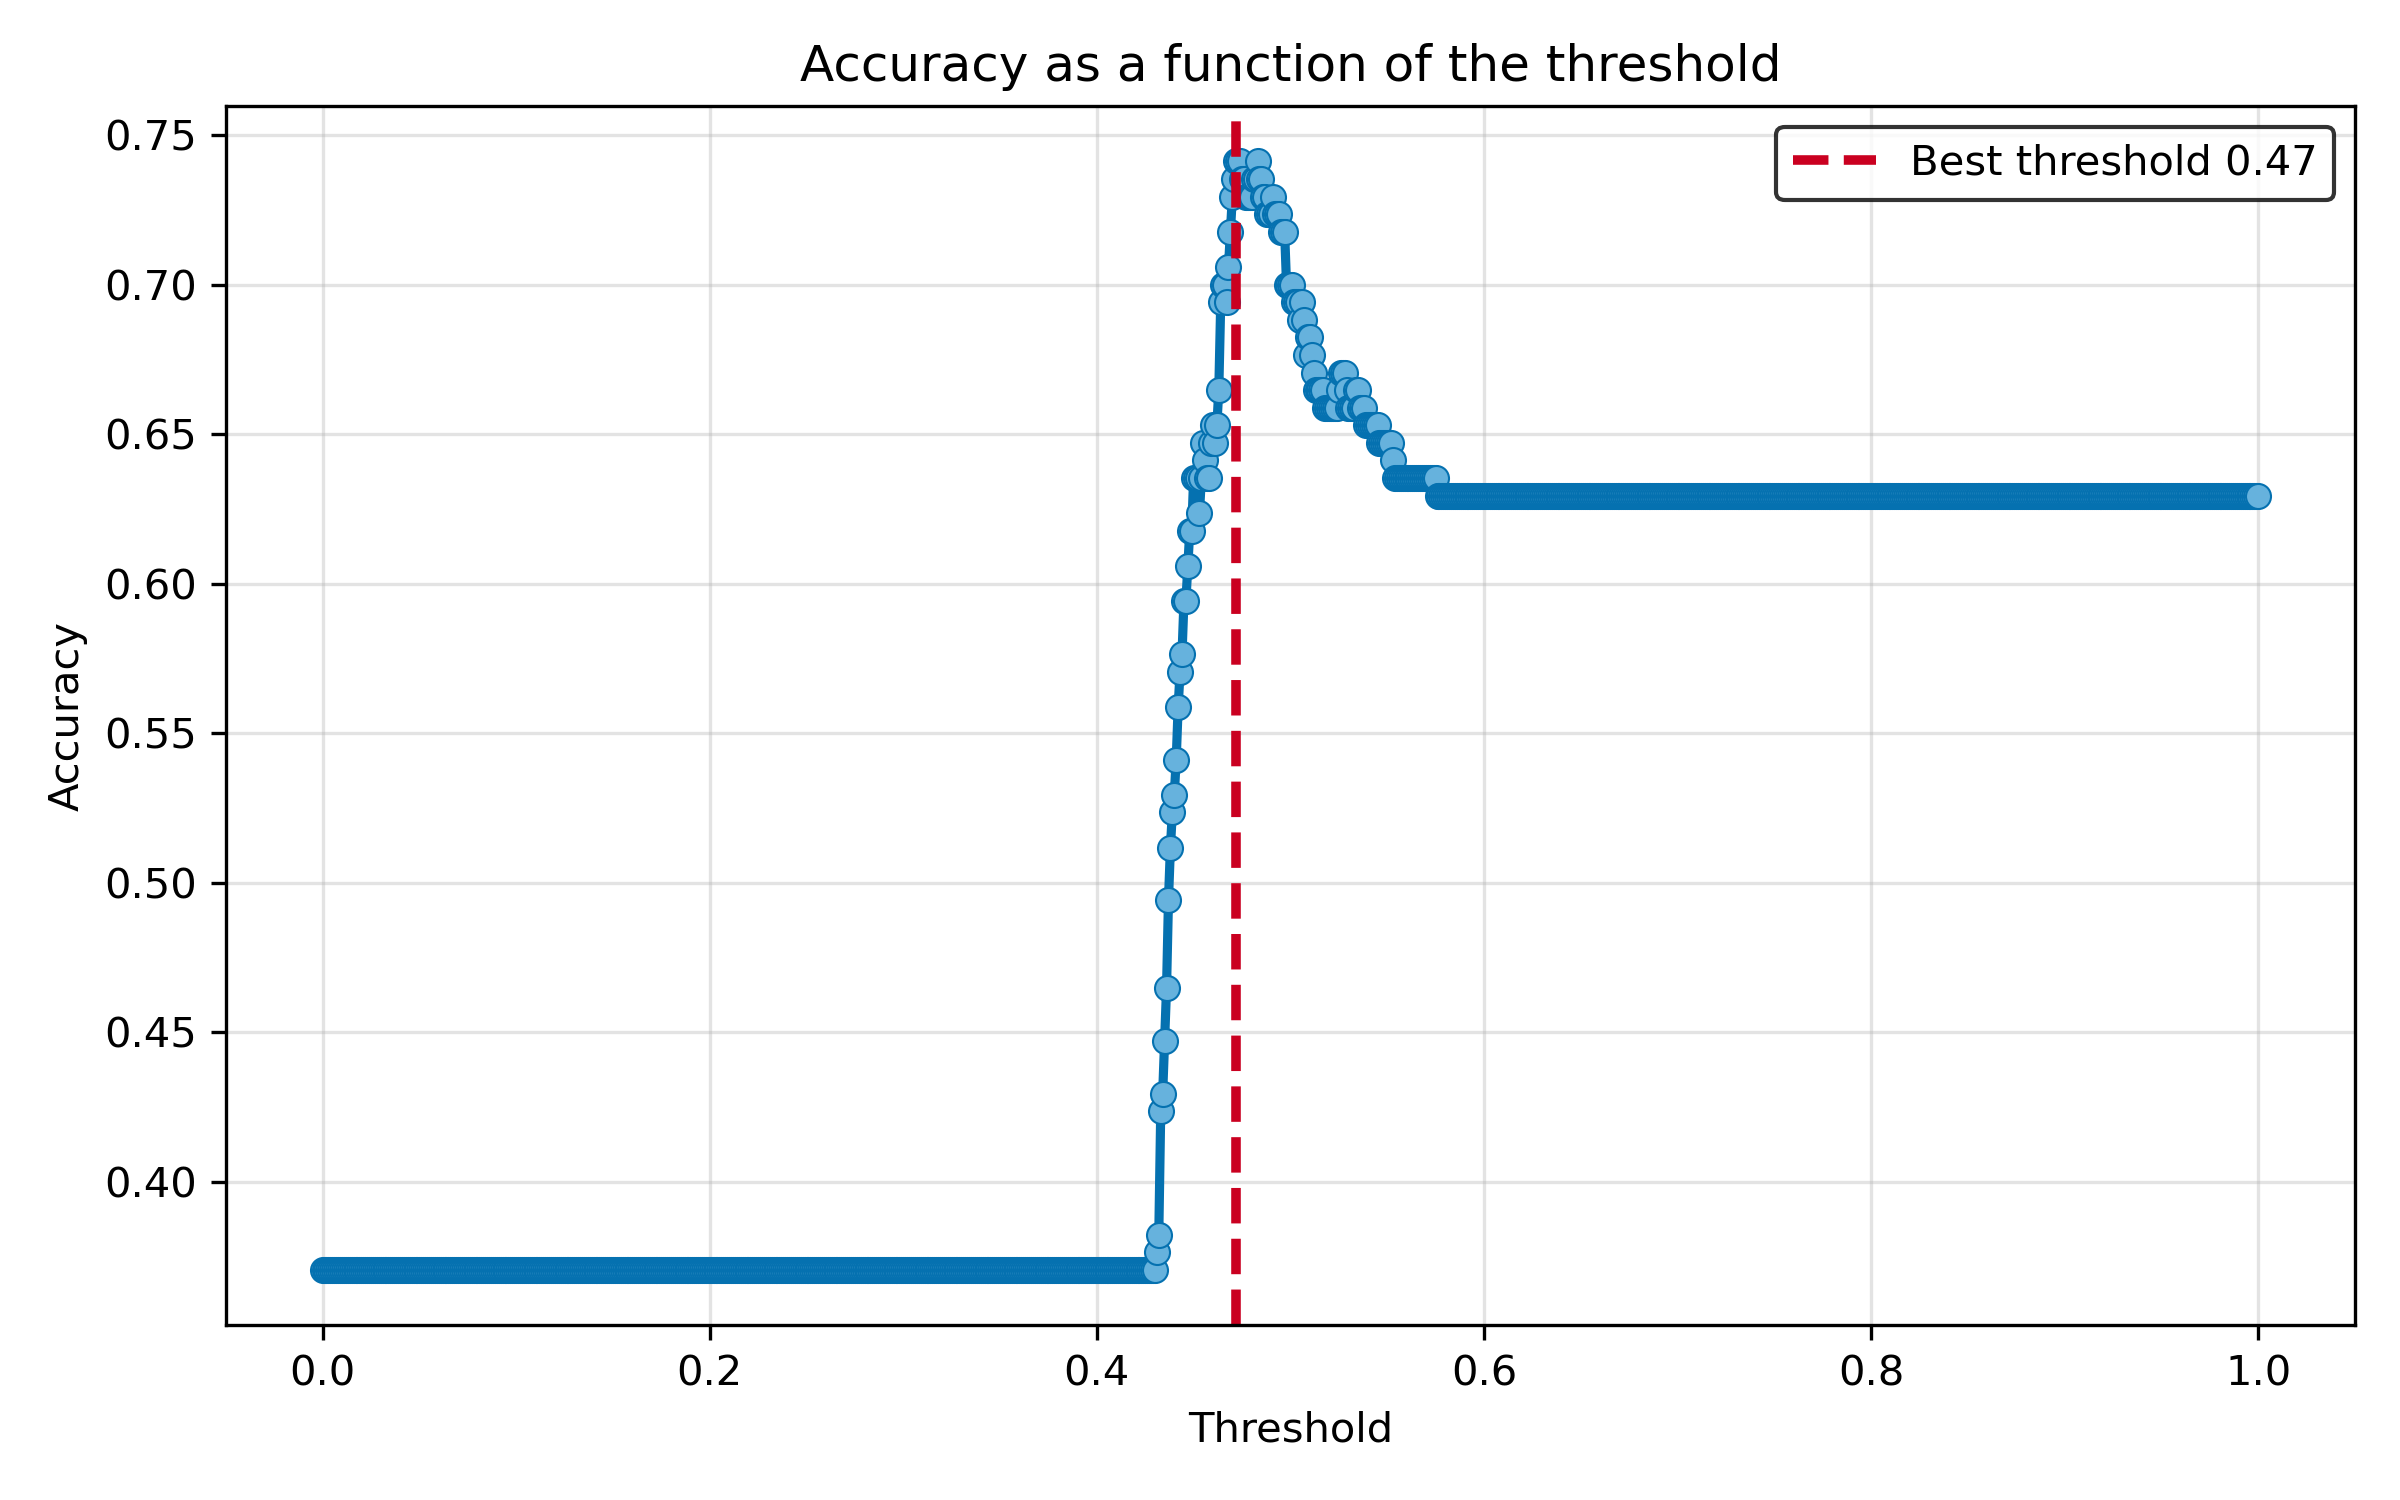
\includegraphics[width=\columnwidth]{figures/accuracy_umbral.png}
		\caption{Accuracy by threshold value $\tau$.}
		\label{fig:accuracy-umbral}
	\end{figure}
	
	The appropriate definition of this threshold is crucial: if the threshold were lower, weak semantic associations would be included; if it were higher, fragments containing substantive references to science would be excluded. Applying $\tau = 0.47$ to the 170 manually evaluated fragments yields an accuracy close to $0.74$, meaning that approximately 74\% of the automatic decisions coincide with the classification obtained through close reading. With the selected threshold, the procedure was applied to the full set of $62{,}651$ corpus fragments, resulting in the identification of a subcorpus composed of $7{,}267$ chunks that meet the criterion of an effective mention of science.
	
	\subsection{Descriptive and Exploratory Analyses of the Text}\label{subsec:descriptive}
	
	To characterize the corpus and establish an appropriate foundation for subsequent analyses, a general descriptive procedure was conducted through the calculation of various statistics. These included the total number of words, the number of unique words, as well as the maximum and minimum document length per column.
	
	Additionally, in order to obtain an exploratory approximation of the discursive content, two word clouds were generated: one corresponding to the full corpus and another to the science subcorpus. Their construction involved preprocessing steps including text cleaning, normalization, and tokenization. The word clouds were built from term frequencies, facilitating a preliminary comparison of the predominant vocabularies in each dataset.
	
	Finally, a temporal analysis was conducted based on the calculation of the monthly volume of documents and the identification of those containing science-related mentions, enabling the construction of a chronological series.
	
	\subsection{Entity Analysis -- NER}\label{subsec:ner}
	
	Named Entity Recognition (NER) is a natural language processing task that consists of identifying entities mentioned in a text and classifying them into predefined categories (e.g., persons, locations, or organizations)~\cite{Jehangir2023}. This process plays a fundamental role in a wide range of applications, including social network analysis, semantic annotation, machine translation, question answering systems, automatic text summarization, document classification, spam detection, and opinion mining~\cite{Jehangir2023}.
	
	In this study, a named entity recognition model was applied to the entire corpus, followed by a comparative analysis with the science subcorpus. To this end, the frequency of occurrence of each entity was calculated in both corpora, and a ratio was computed to indicate the extent to which a given entity appears more frequently in science-related texts than in the rest of the corpus.
	
	The model used was \textit{Babelscape/wikineural-multilingual-ner}~\cite{tedeschi-etal-2021-wikineural-combined}, available in the Sentence Transformers library. This model exhibits strong performance metrics and is pre-trained on multilingual data that include Spanish. It recognizes locations, persons, and organizations.
	
	\subsection{Analysis of Topics}\label{subsec:topics}
	
	Once the science-related mentions had been identified and the corresponding subcorpus constructed, topic modeling was conducted in order to infer the latent thematic structures present in both the general corpus and the science subcorpus. Topic modeling comprises a set of unsupervised methods aimed at discovering recurrent semantic patterns within a collection of documents~\cite{Abdelrazek2023}. Conceptually, these methods seek to model three fundamental entities: the document collection, the latent topics, and the constructs that compose them.
	
	From a mathematical standpoint, a topic can be understood as a probability distribution over the vocabulary of the corpus. That is, given a set of words $w_1, w_2, \dots, w_V$ that constitute the vocabulary, a topic $k$ is represented as a probability vector:
	\[
	\boldsymbol{\phi}_k = \bigl( P(w_1 \mid k), P(w_2 \mid k), \dots, P(w_V \mid k) \bigr),
	\]
	where $P(w_v \mid k) \ge 0$ and $\sum_{v=1}^{V} P(w_v \mid k) = 1$.
	
	The literature identifies four major families of methods for topic modeling: algebraic, fuzzy, probabilistic, and neural. Among neural approaches, BERTopic~\cite{Grootendorst2022} stands out, as it combines pre-trained embeddings, dimensionality reduction, and clustering algorithms to identify groups of documents with high semantic proximity.
	
	Since embeddings had already been used in earlier stages of the analysis to represent corpus fragments, methodological coherence was maintained by employing the same vector representation model (\texttt{embeddinggemma-300m}) for topic modeling. The model was applied to both the full corpus and the science subcorpus, enabling subsequent comparisons between general thematic configurations and those specifically associated with scientific discourse.
	
	To evaluate the quality of the estimated topics, the topic coherence metric was used. This measure, based on probabilistic principles of term co-occurrence, has been shown to correlate positively with human interpretability of topics~\cite{Rder2015}. In order to select the optimal number of topics, the model was run with different parameter values, and the corresponding coherence was calculated in each case. The value that maximized this metric was adopted as the final configuration of the model.
	
	\subsection{Vocabulary Analysis with POS-Tagging}\label{subsec:pos}
	
	In order to identify the most relevant vocabulary associated with scientific discourse in opinion columns, a frequency analysis of verbs, adjectives, and nouns was conducted for both the general corpus and the science subcorpus. To obtain these grammatical categories, a Part-of-Speech Tagging (POS-tagging) model was employed. This task consists of assigning each word its corresponding syntactic category~\cite{he2020surveyrecentadvancessequence}. POS-tagging constitutes a fundamental component in various natural language processing applications, such as machine translation, information retrieval and extraction, syntactic parsing, semantic disambiguation, and sentiment analysis~\cite{Chiche2022}.
	
	For this study, the Stanza POS-tagger was used. Stanza is a Python-based linguistic analysis package that includes models trained for multiple languages, including Spanish~\cite{qi2020stanza}. This model was selected due to its reported performance metrics and its suitability for journalistic texts. In the analyzed corpus, it exhibited consistent behavior, enabling the reliable extraction of the grammatical classes required for the comparative frequency analysis.
	
	%%---------------------------------------------------------
	%%  SECTION 3 ? RESULTS
	%%---------------------------------------------------------
	\section{Results}\label{sec:results}
	
	In this section, the results derived from the methodological procedure described above are presented, following the same analytical sequence. First, the identification of effective mentions of science and the delimitation of the corresponding subcorpus are reported. Subsequently, descriptive and exploratory analyses are presented to quantitatively characterize its presence within the corpus. Next, the results of the named entity recognition task are introduced in order to identify actors and institutions associated with scientific discourse. This is followed by the findings of the topic modeling, which allow the inference of latent thematic structures in both the general corpus and the science subcorpus. Finally, lexical and grammatical patterns are analyzed through POS-tagging techniques.
	
	\subsection{Identification of Mentions of Science}\label{subsec:mentions}
	
	Based on the manual classification of 170 fragments used for validation, an appropriate threshold was determined to be $\tau = 0.47$, yielding an \emph{accuracy} of 0.741. Once this criterion was established, the procedure was applied to the full set of 13,676 opinion columns, which had been segmented into 62,651 fragments. Of these, 7,267 fragments were identified as related to science, representing 11.6\% of the total number of fragments.
	
	At the document level, 4,154 columns contain at least one effective mention of science, corresponding to 30.4\% of the total number of analyzed columns. Table~\ref{tab:res_fragmentos_subcategoria} presents the distribution of fragments classified as scientific mentions across the 17 categories of the UNESCO Thesaurus.
	
	\begin{table}[t]
		\caption{Number of fragments with mentions of science and percentage of the total by category.}
		\label{tab:res_fragmentos_subcategoria}
		{\footnotesize
			\begin{tabular}{@{}p{4.2cm}cc@{}}
				\toprule
				\textbf{Category} & \textbf{Fragments} & \textbf{\%} \\
				\midrule
				Science and research management    & 3195 & 43.97 \\
				Pollution, disasters and safety    & 1566 & 21.55 \\
				Environmental sciences/engineering & 635  & 8.74  \\
				Natural sciences                   & 470  & 6.47  \\
				Pathology                          & 375  & 5.16  \\
				Medical sciences                   & 306  & 4.21  \\
				Mathematics and statistics         & 250  & 3.44  \\
				Hydrology                          & 104  & 1.43  \\
				Natural resources                  & 68   & 0.94  \\
				Scientific approach                & 64   & 0.88  \\
				Space sciences                     & 61   & 0.84  \\
				Geography and oceanography         & 49   & 0.67  \\
				Biology                            & 36   & 0.50  \\
				Meteorology                        & 28   & 0.39  \\
				Earth sciences                     & 23   & 0.32  \\
				Physical sciences                  & 20   & 0.28  \\
				Chemical sciences                  & 17   & 0.23  \\
				\midrule
				\textbf{Total}                     & \textbf{7267} & \textbf{100} \\
				\botrule
			\end{tabular}
		}
	\end{table}
	
	\subsection{Descriptive and Exploratory Analyses}\label{subsec:descriptive_results}
	
	\begin{table}[t]
		\caption{General descriptive statistics of the corpus.}
		\label{tab:estadisticos_generales}
		\begin{tabular}{@{}lc@{}}
			\toprule
			\textbf{Statistic} & \textbf{Value} \\
			\midrule
			Total number of documents           & 13676   \\
			Total words                         & 8607473 \\
			Average words per document          & 629     \\
			Median words per document           & 590     \\
			Maximum words per document          & 5223    \\
			Minimum words per document          & 128     \\
			Number of distinct authors          & 584     \\
			Number of distinct media outlets    & 3       \\
			Number of unique words (vocabulary) & 283923  \\
			\botrule
		\end{tabular}
	\end{table}
	
	\begin{figure}[t]
		\centering
		\begin{subfigure}{\columnwidth}
			\centering
			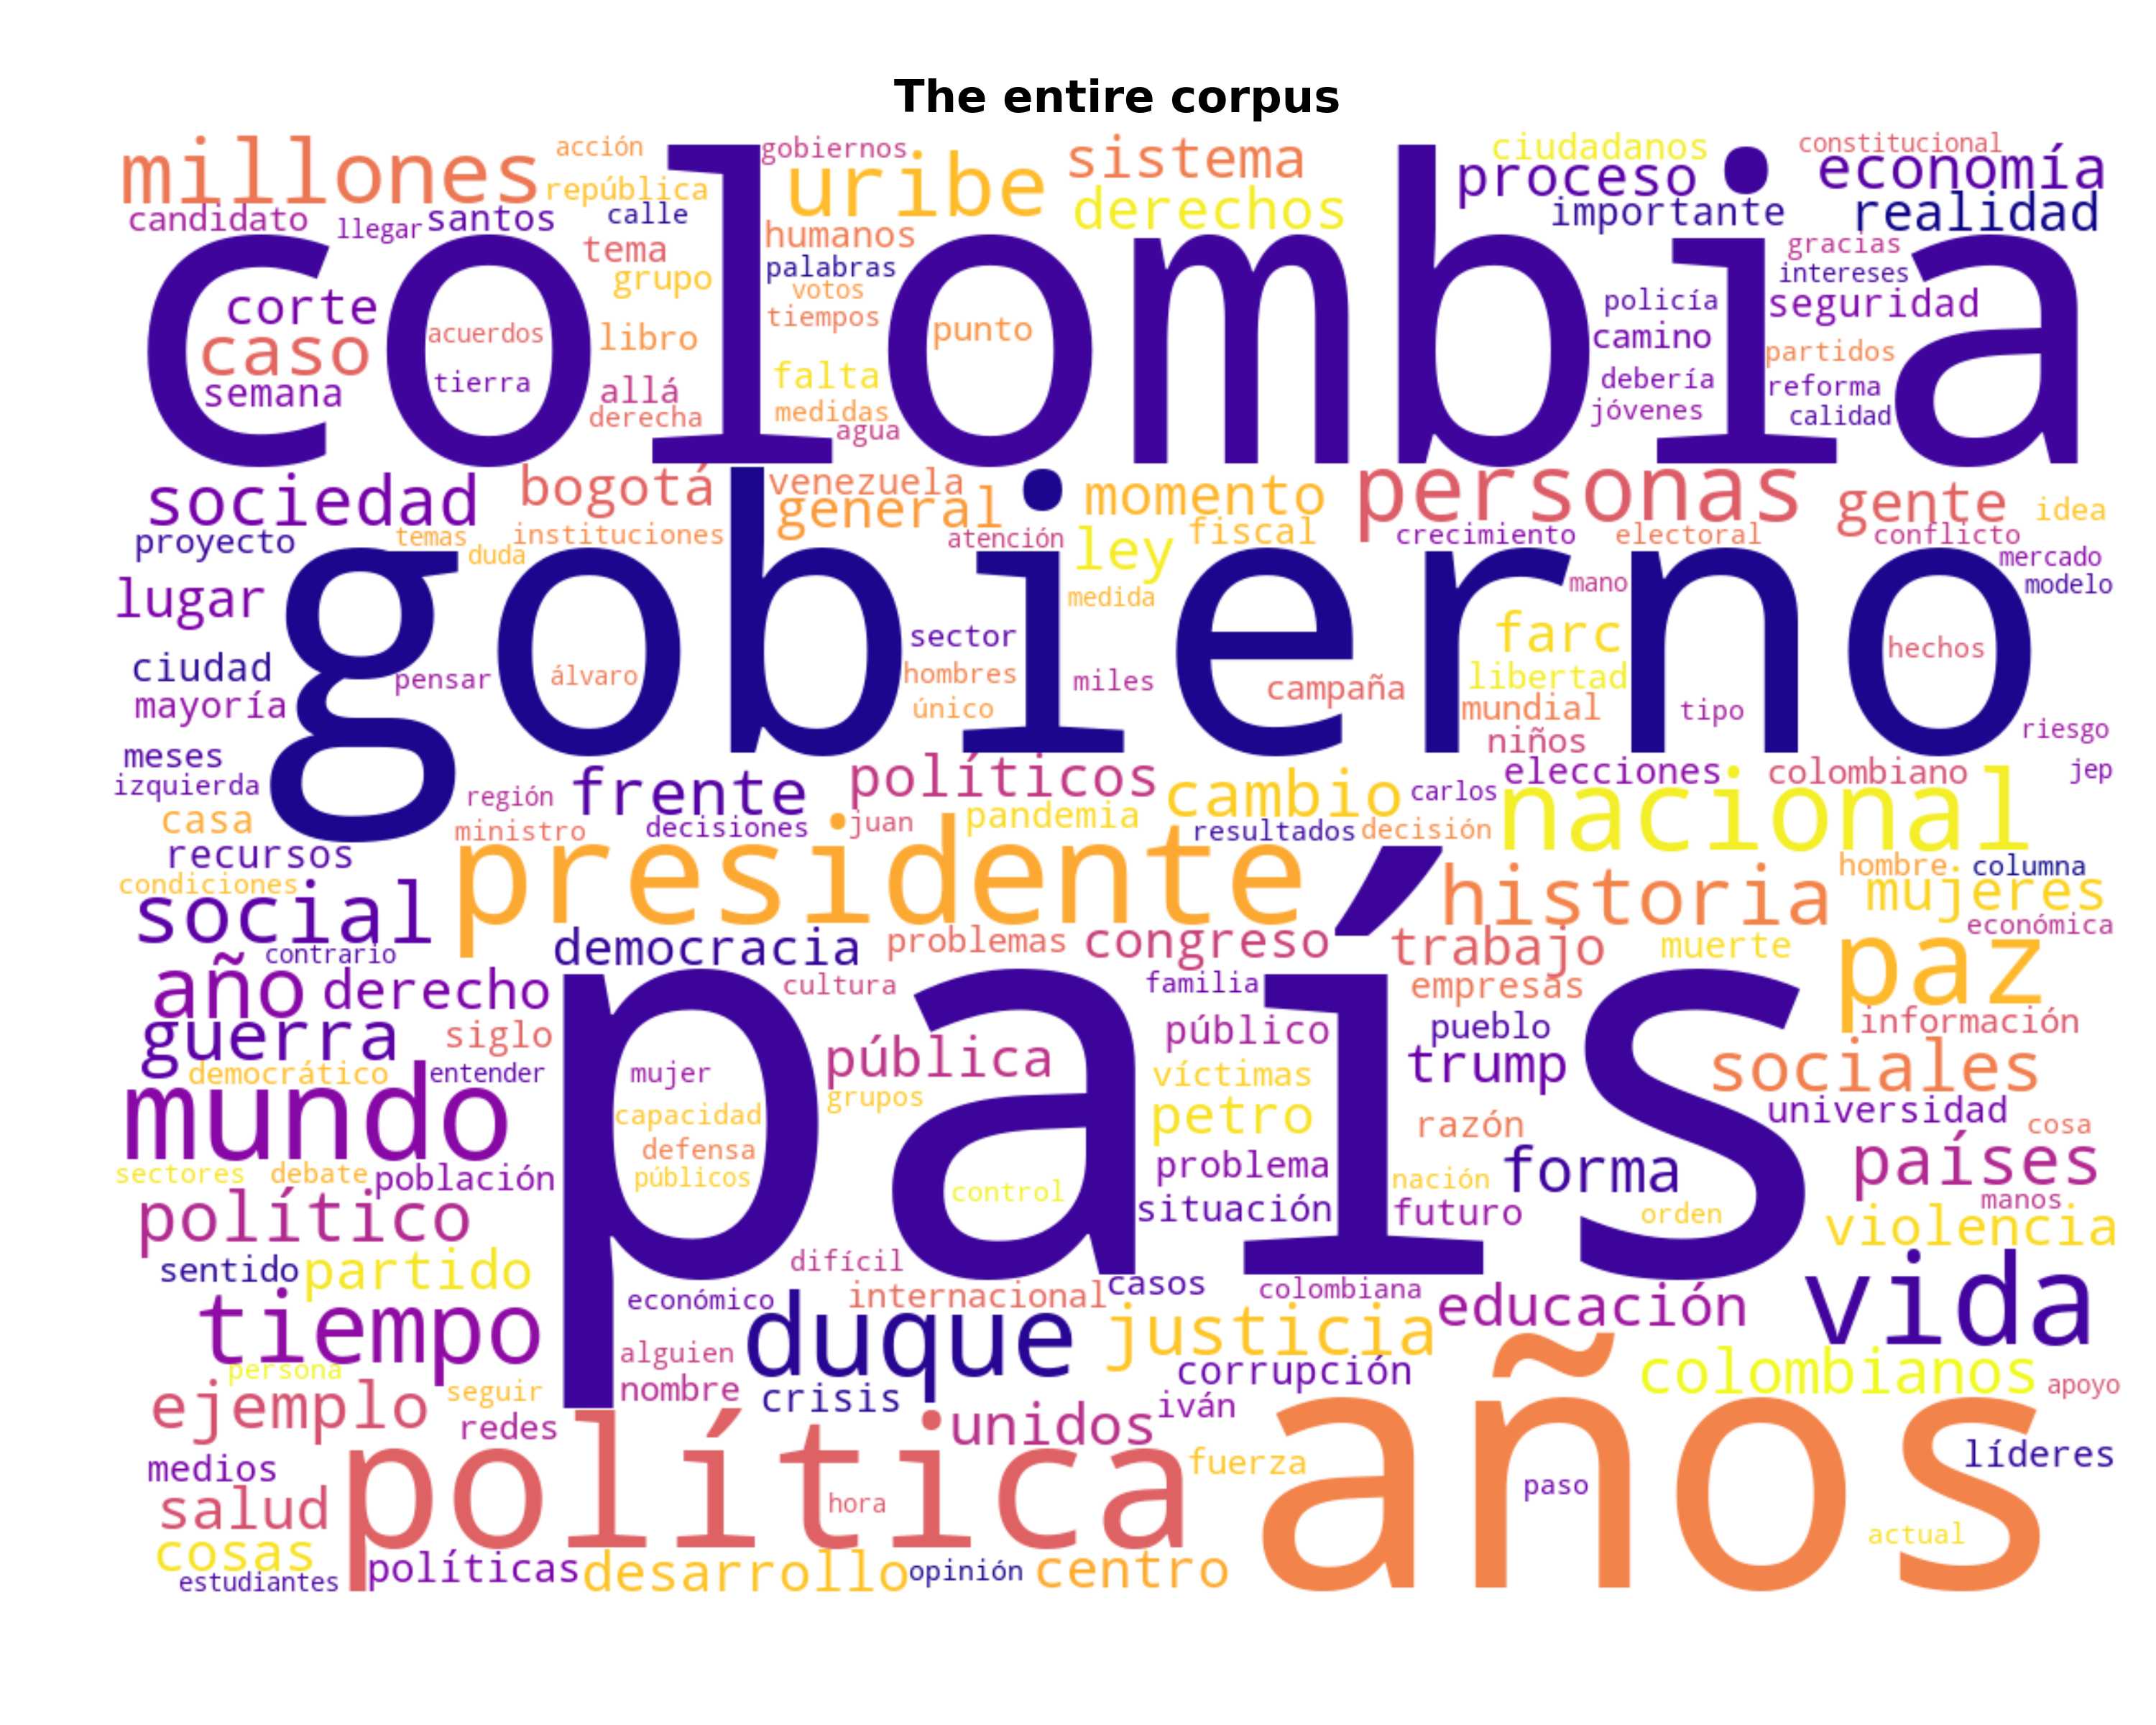
\includegraphics[width=\columnwidth]{figures/nube_general.png}
			\caption{Word cloud of the general corpus.}
			\label{fig:nube_general}
		\end{subfigure}
		\begin{subfigure}{\columnwidth}
			\centering
			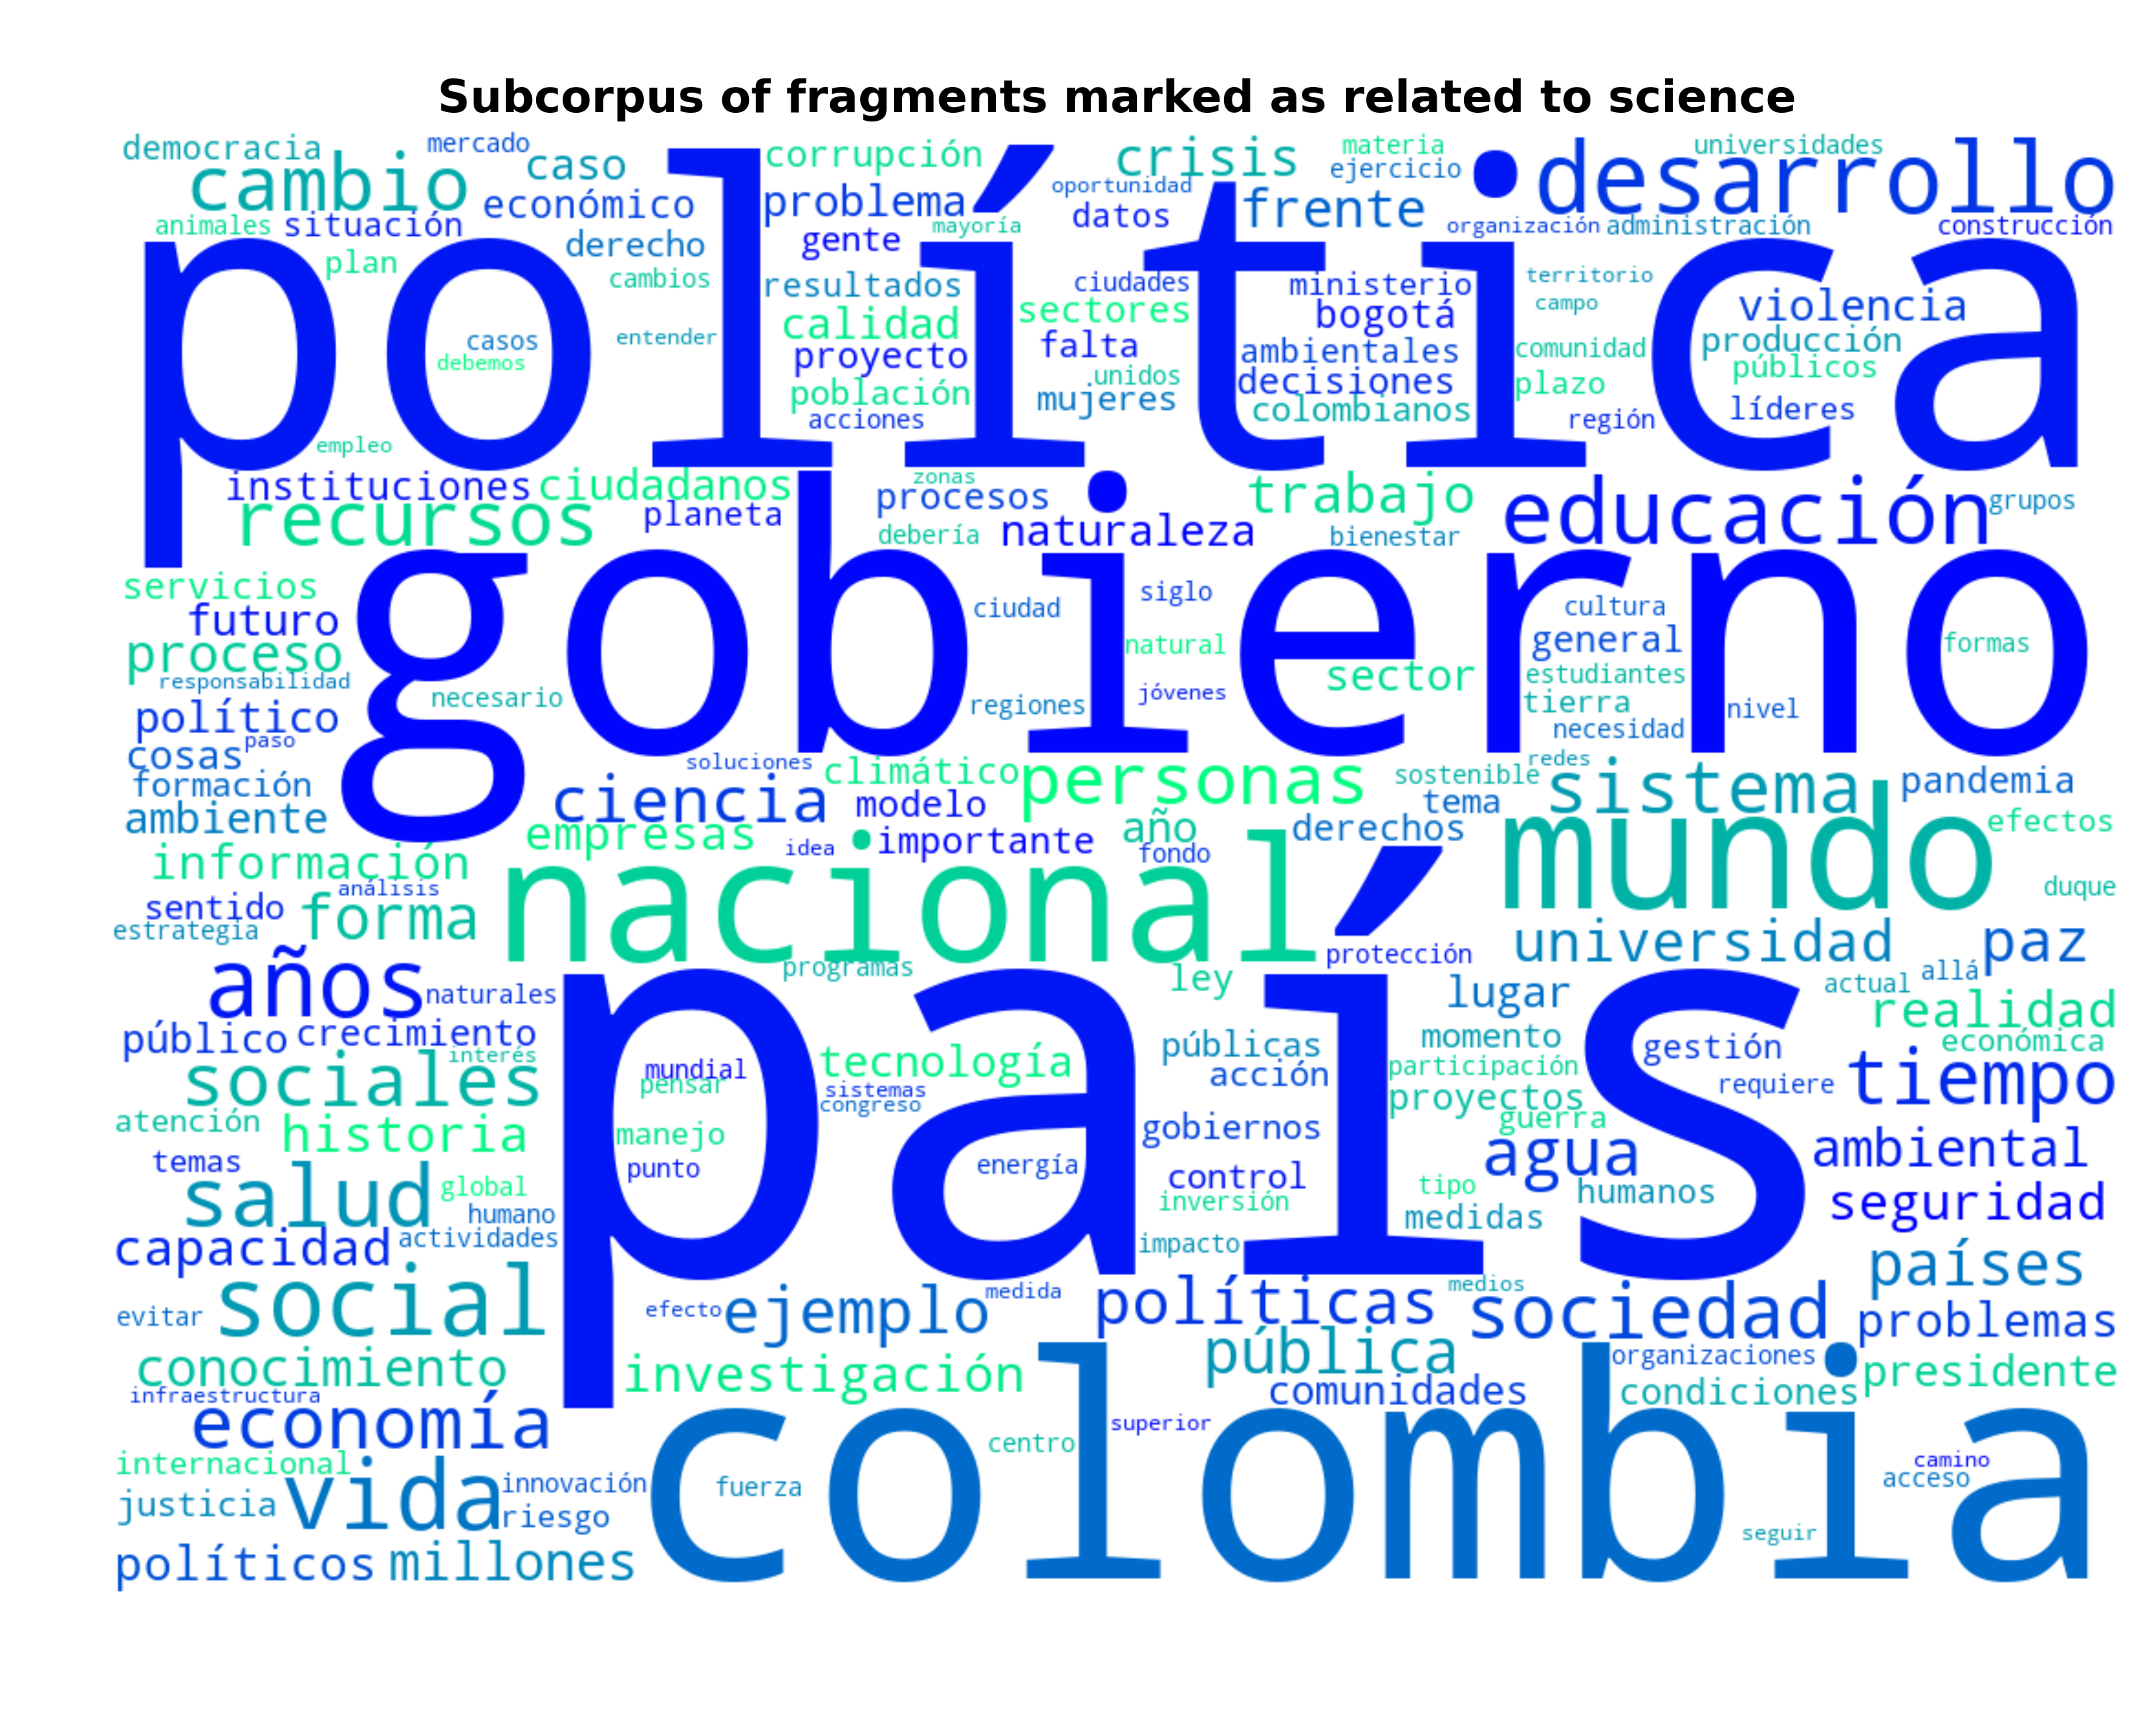
\includegraphics[width=\columnwidth]{figures/nube_ciencia.png}
			\caption{Word cloud of the science subcorpus.}
			\label{fig:nube_ciencia}
		\end{subfigure}
		\caption{Word clouds comparing predominant vocabulary in the general corpus versus the subcorpus.}
		\label{fig:nube_comparativa}
	\end{figure}
	
	Figure~\ref{fig:dist_mensual_ciencia} shows, for each month in the analyzed period, the percentage of columns containing at least one effective mention of science relative to the total number of columns published in that month. A notable increase can be observed in March and April 2020, the months with the highest proportion of mentions, suggesting a direct association between the intensification of scientific discourse and the onset of the COVID-19 pandemic.
	
	\begin{figure}[t]
		\centering
		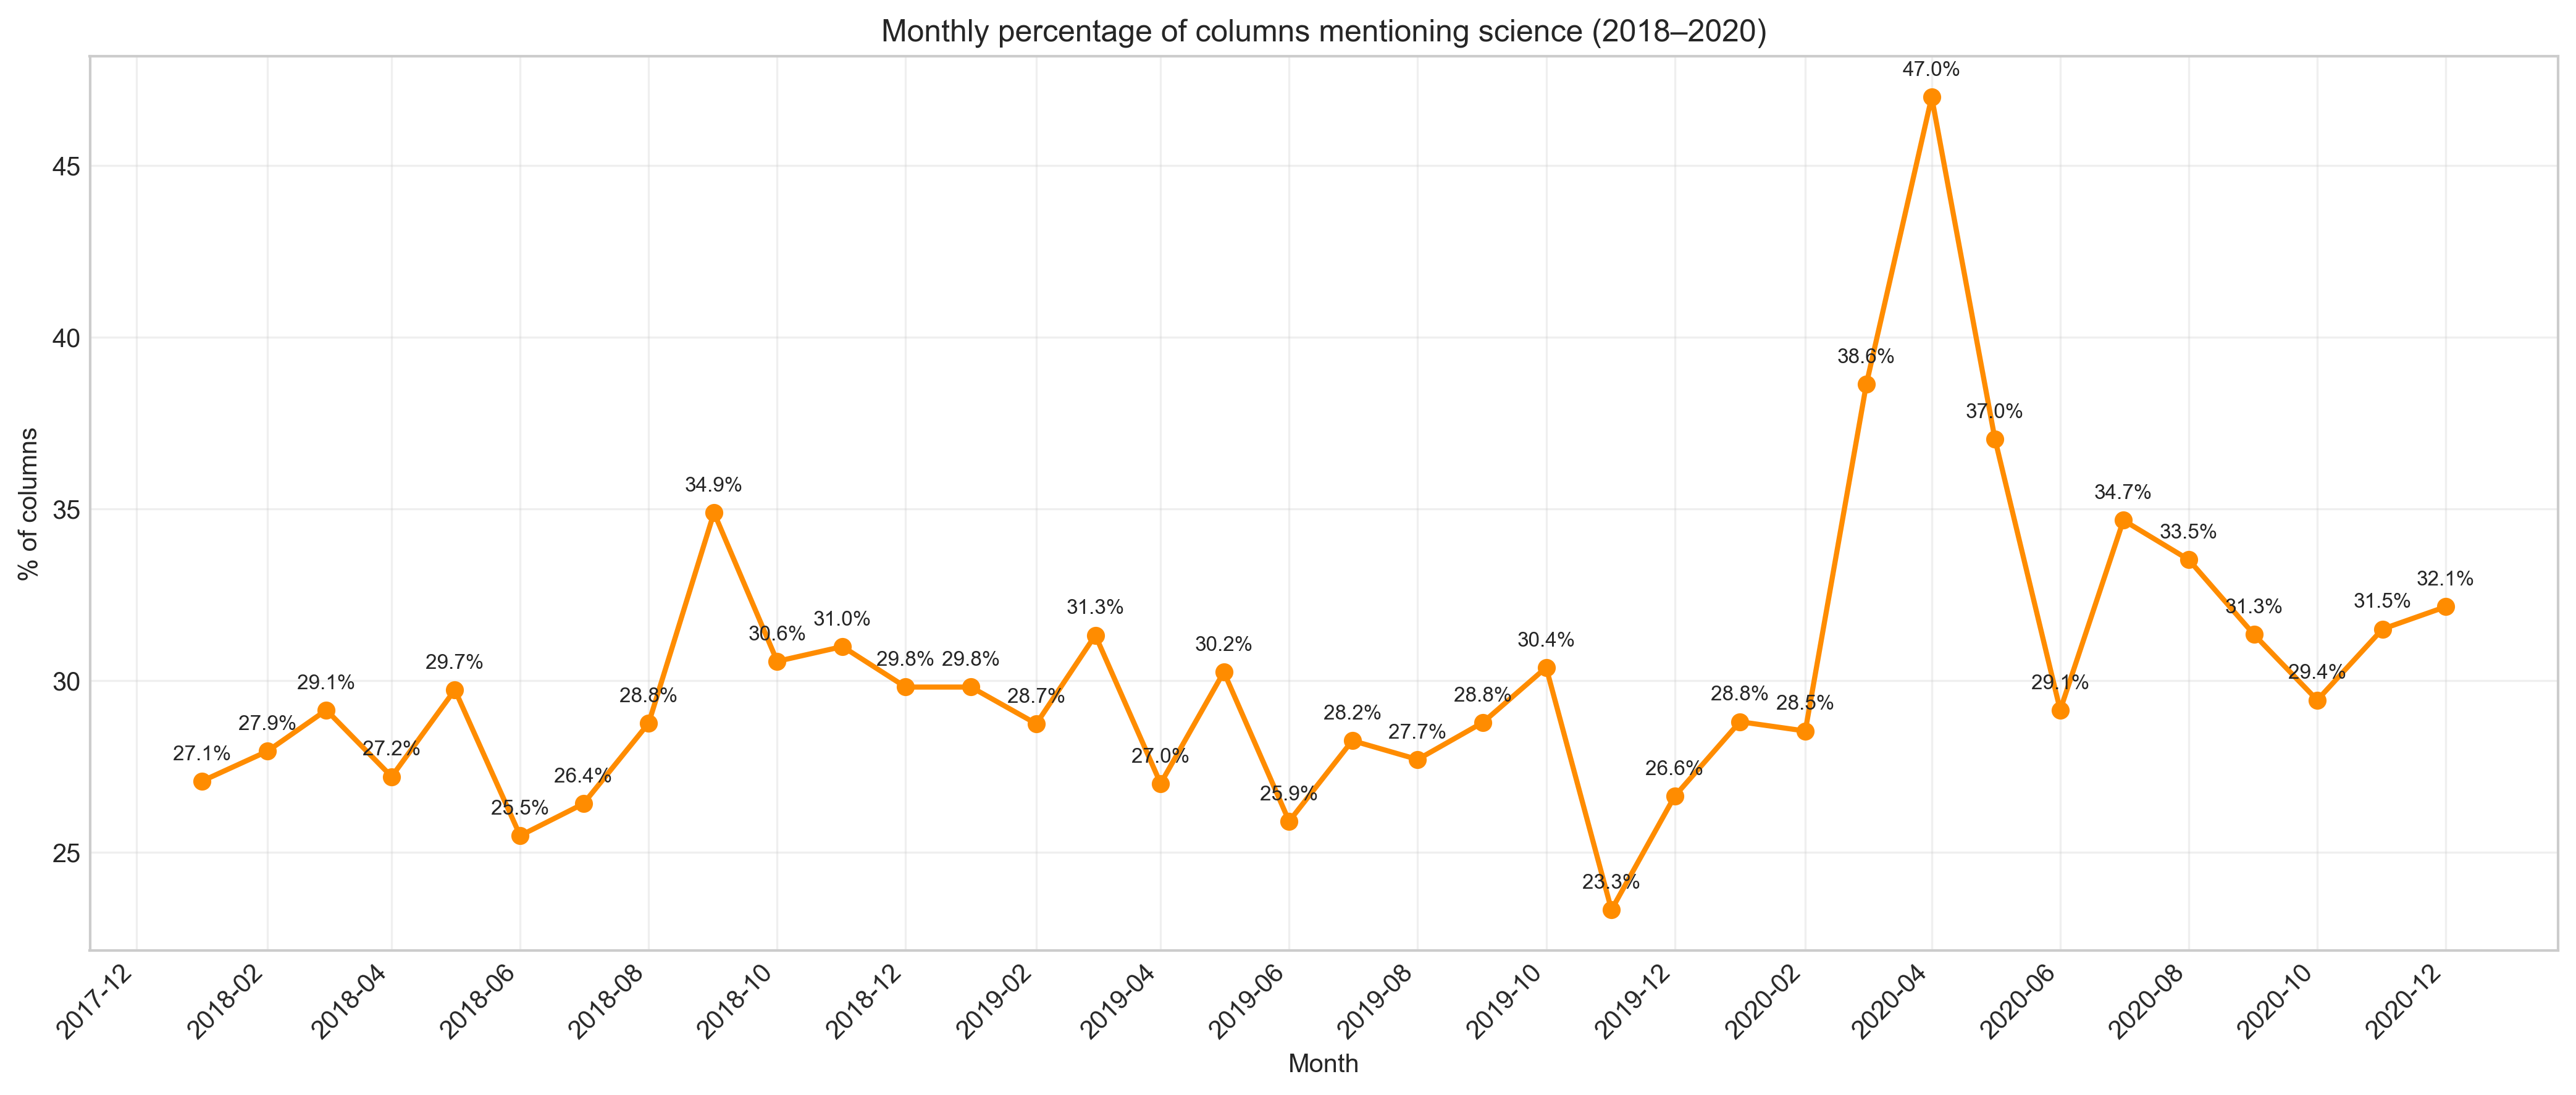
\includegraphics[width=\columnwidth]{figures/porcentaje_mensual_ciencia_linea.png}
		\caption{Monthly distribution of columns mentioning science, by percentage.}
		\label{fig:dist_mensual_ciencia}
	\end{figure}
	
	\subsection{Named Entity Recognition}\label{subsec:ner_results}
	
	The ten most frequent entities by class (Person, Organization, and Location) are presented below, considering only those whose occurrence exceeds 30\% of the subcorpus of fragments with effective mentions of science. This criterion makes it possible to focus the analysis on the actors, institutions, and geographic spaces with the greatest centrality in the scientific discourse of opinion columns.
	
	\begin{table*}[t]
		\caption{Comparative frequency of persons in the general corpus vs.\ the scientific corpus.}
		\label{tab:ents_per}
		{\footnotesize
			\begin{tabular}{@{}p{2.8cm}cccP{5cm}@{}}
				\toprule
				\textbf{Entity (PER)} & \textbf{Corpus Freq.} & \textbf{Science Freq.} & \textbf{\% Sci./Corp.} & \textbf{Description} \\
				\midrule
				Humboldt              & 63 & 23 & 36 & German naturalist, geographer and explorer, 18th--19th c. \\
				Newton                & 25 & 9  & 36 & English physicist, 17th--18th c. \\
				Stephen Hawking       & 41 & 16 & 39 & British scientist and science communicator, 20th--21st c. \\
				Charles Darwin        & 25 & 11 & 44 & English naturalist, 19th c. \\
				Greta Thunberg        & 50 & 16 & 32 & Swedish environmental activist, 21st c. \\
				Ricardo Lozano        & 15 & 7  & 46 & Geologist and former Minister of Environment and Sustainable Development of Colombia (2018). \\
				Mabel Torres          & 13 & 7  & 53 & Colombian scientist and former Minister of Science, Technology and Innovation (2020). \\
				Wade Davis            & 12 & 4  & 33 & Canadian-Colombian scientist. \\
				Dolly Montoya Casta{\~n}o & 12 & 4 & 33 & Colombian scientist and former rector of the National University of Colombia. \\
				Carl Sagan            & 10 & 5  & 50 & American astronomer, astrophysicist and science communicator, 20th c. \\
				\botrule
			\end{tabular}
		}
	\end{table*}
	
	\begin{table*}[t]
		\caption{Comparative frequency of organizations in the general corpus vs.\ the scientific corpus.}
		\label{tab:ents_org}
		{\footnotesize
			\begin{tabular}{@{}p{3.5cm}cccP{5cm}@{}}
				\toprule
				\textbf{Entity (ORG)} & \textbf{Corpus Freq.} & \textbf{Science Freq.} & \textbf{\% Sci./Corp.} & \textbf{Description} \\
				\midrule
				OECD                             & 296 & 86 & 30 & Organisation for Economic Co-operation and Development. \\
				Universidad Pedag{\'o}gica Nacional & 117 & 55 & 47 & Public university in Colombia. \\
				Pontificia Universidad Javeriana & 103 & 33 & 32 & Private university in Colombia. \\
				Ministry of Agriculture          & 111 & 33 & 30 & Colombian ministry responsible for the agricultural, fisheries and rural development sector. \\
				Colciencias                      & 74  & 47 & 63 & Former entity responsible for promoting public policies in science, technology and innovation in Colombia. Replaced by Minciencias in 2019. \\
				Ministry of Environment and Sustainable Development & 70 & 41 & 59 & Colombian ministry responsible for environmental policy. \\
				University of Massachusetts Amherst & 49 & 21 & 42 & Public university and research center in the United States. \\
				Finagro                          & 44  & 15 & 34 & Fund for the financing of the agricultural sector in Colombia. \\
				IDEAM                            & 40  & 24 & 60 & Institute of Hydrology, Meteorology and Environmental Studies of Colombia. \\
				FAO                              & 40  & 15 & 37 & Food and Agriculture Organization of the United Nations. \\
				\botrule
			\end{tabular}
		}
	\end{table*}
	
	\begin{table*}[t]
		\caption{Comparative frequency of locations in the general corpus vs.\ the scientific corpus.}
		\label{tab:ents_loc}
		{\footnotesize
			\begin{tabular}{@{}p{3cm}cccP{5.5cm}@{}}
				\toprule
				\textbf{Entity (LOC)} & \textbf{Corpus Freq.} & \textbf{Science Freq.} & \textbf{\% Sci./Corp.} & \textbf{Description} \\
				\midrule
				Colombia        & 16017 & 2066 & 39 & South American country, official language Spanish. \\
				Bogot{\'a}      & 2745  & 778  & 28 & Capital of Colombia. \\
				Latin America   & 1690  & 571  & 34 & Region comprising Spanish- and Portuguese-speaking countries south of the US. \\
				Amazon          & 710   & 373  & 53 & Biogeographical region covering the Amazon River basin. \\
				Medell{\'i}n    & 1127  & 308  & 27 & Second largest city of Colombia; capital of the department of Antioquia. \\
				Pacific         & 598   & 290  & 49 & Region corresponding to the Colombian Pacific coast. \\
				Orinoquia       & 308   & 193  & 63 & Biogeographical region in eastern Colombia. \\
				Cali            & 715   & 213  & 30 & Third largest city of Colombia. \\
				Paris           & 619   & 207  & 33 & Capital of France. \\
				Andes           & 396   & 195  & 49 & Mountain range crossing South America from north to south. \\
				\botrule
			\end{tabular}
		}
	\end{table*}
	
	\subsection{Analysis of Topics}\label{subsec:topic_results}
	
	Topic modeling was first applied to the full corpus. Table~\ref{tab:bertopic_nr_topics_all} presents the results of BERTopic for different values of \texttt{num\_topics}, and Table~\ref{tab:bertopic_coherence_top} shows the top topics of the selected model.
	
	\begin{table}[t]
		\caption{BERTopic results for different values of \texttt{num\_topics}, full corpus.}
		\label{tab:bertopic_nr_topics_all}
		\begin{tabular}{@{}cccc@{}}
			\toprule
			\textbf{num\_topics} & \textbf{Final topics} & \textbf{Coherence $c_v$} & \textbf{\% Outliers} \\
			\midrule
			auto & 38 & 0.722461 & 0.0 \\
			20   & 19 & 0.715830 & 0.0 \\
			30   & 25 & 0.711820 & 0.0 \\
			40   & 35 & 0.707073 & 0.0 \\
			60   & 47 & 0.698219 & 0.0 \\
			10   & 9  & 0.674196 & 0.0 \\
			\botrule
		\end{tabular}
	\end{table}
	
	\begin{table*}[t]
		\caption{Top BERTopic topics with per-topic coherence ($c_v$), percentage of documents, and representative keywords (full corpus).}
		\label{tab:bertopic_coherence_top}
		\begin{tabularx}{\textwidth}{@{}cccX@{}}
			\toprule
			\textbf{Topic} & \textbf{Coherence ($c_v$)} & \textbf{\%} & \textbf{Keywords} \\
			\midrule
			0  & 0.5509 & 40.06 & president, government, duque, peace, country, uribe, colombia, politics, years, petro \\
			2  & 0.8437 & 5.58  & economy, taxes, growth, income, fiscal, companies, rate, employment, gdp, deficit \\
			1  & 0.7322 & 5.27  & pandemic, virus, health, coronavirus, covid19, world, quarantine, measures, crisis, people \\
			3  & 0.8185 & 4.25  & education, students, university, universities, quality, training, higher, national, teachers, schools \\
			4  & 0.8427 & 3.34  & women, woman, men, sexual, violence, gender, sex, feminism, harassment \\
			7  & 0.6890 & 2.53  & networks, information, data, facebook, media, social, communication, people, internet, twitter \\
			8  & 0.7879 & 2.23  & hectares, rural, deforestation, land, agriculture, producers, agricultural, crops, development \\
			5  & 0.8642 & 2.13  & football, players, team, game, teams, cup, national team, sport, goal, world cup \\
			20 & 0.5990 & 2.05  & corruption, corrupt, public, referendum, anti-corruption, fight, officials, resources, country, politics \\
			6  & 0.8998 & 1.61  & cuisine, food, eat, restaurant, dish, flavors, rice, dishes, flavor, home \\
			\botrule
		\end{tabularx}
	\end{table*}
	
	The same procedure was applied to fragments classified as references to science. Table~\ref{tab:bertopic_nr_topics_ciencia} presents the results for different parameter values; the best model among those evaluated was the one with 20 topics. For this model, the results are presented in Table~\ref{tab:topics_ciencia}. Ninety percent of the documents were concentrated in the first 10 topics, indicating high thematic concentration.
	
	\begin{table}[t]
		\caption{BERTopic results for different values of \texttt{num\_topics}, science subcorpus.}
		\label{tab:bertopic_nr_topics_ciencia}
		\begin{tabular}{@{}cccc@{}}
			\toprule
			\textbf{num\_topics} & \textbf{Final topics} & \textbf{Coherence $c_v$} & \textbf{\% Outliers} \\
			\midrule
			20   & 19 & 0.695491 & 0.0 \\
			40   & 28 & 0.695162 & 0.0 \\
			auto & 26 & 0.694176 & 0.0 \\
			30   & 28 & 0.681233 & 0.0 \\
			60   & 27 & 0.678842 & 0.0 \\
			10   & 9  & 0.622583 & 0.0 \\
			\botrule
		\end{tabular}
	\end{table}
	
	\begin{table*}[t]
		\caption{Top BERTopic topics with per-topic coherence ($c_v$), percentage of documents, and representative keywords (science subcorpus).}
		\label{tab:topics_ciencia}
		\begin{tabularx}{\textwidth}{@{}cccX@{}}
			\toprule
			\textbf{Topic} & \textbf{Coherence ($c_v$)} & \textbf{\%} & \textbf{Keywords} \\
			\midrule
			1  & 0.493785 & 25.62 & politics, government, peace, country, security, violence, political, politicians, justice, colombia \\
			0  & 0.460526 & 21.69 & health, world, life, pandemic, time, science, people, virus, years, crisis \\
			3  & 0.574302 & 11.42 & economy, development, growth, resources, country, sector, government, politics, fiscal, innovation \\
			2  & 0.782987 & 9.61  & education, university, training, universities, students, national, quality, research, knowledge, higher \\
			4  & 0.784604 & 6.56  & environmental, conservation, environment, biodiversity, sustainable, development, deforestation, forests, ecosystems \\
			5  & 0.799532 & 4.79  & climate, change, planet, global, warming, wildfires, world, climatic, weather, temperature \\
			8  & 0.504077 & 2.79  & data, information, surveys, access, transparency, results, people, media, example, public \\
			7  & 0.686045 & 2.75  & water, river, waters, rain, rivers, cauca, neighborhoods, works, bogot{\'a}, country \\
			9  & 0.919135 & 2.02  & energy, fuels, fossil, energies, coal, renewables, solar, energetic, oil, gas \\
			10 & 0.724657 & 1.83  & women, men, woman, gender, feminine, violence, people, life, female, sex \\
			\botrule
		\end{tabularx}
	\end{table*}
	
	\subsection{Vocabulary Analysis with POS-Tagging}\label{subsec:pos_results}
	
	Verbs, adjectives, and nouns were extracted from the corpus using POS-tagging techniques, and their frequencies were calculated. In total, approximately 10,000 verbs, 18,000 adjectives, and 30,000 different nouns were identified. In the complete corpus, the most frequent verb is \textit{have}, the most frequent adjective is \textit{social}, and the most frequent noun is \textit{country}. These same words also top the frequency lists in the science subcorpus.
	
	Given that 11.6\% of the fragments in the corpus were classified as scientific mentions, those words whose proportion of occurrence in the science subcorpus exceeds that percentage were selected. This criterion allows us to identify terms with a relatively greater presence in scientific discourse compared to the general corpus.
	
	\begin{table}[t]
		\caption{Frequency and proportion of verbs in the science subcorpus.}
		\label{tab:verbos_ciencia}
		\begin{tabular}{@{}lrrr@{}}
			\toprule
			\textbf{Verb} & \textbf{Total} & \textbf{Science} & \textbf{Proportion} \\
			\midrule
			\textit{articular} (`articulate')   & 175 & 79 & 0.45 \\
			\textit{mitigar} (`mitigate')       & 208 & 68 & 0.33 \\
			\textit{contaminar} (`contaminate') & 200 & 63 & 0.32 \\
			\textit{gestionar} (`manage')       & 188 & 57 & 0.30 \\
			\textit{actualizar} (`update')      & 122 & 37 & 0.30 \\
			\textit{deforestar} (`deforest')    & 67  & 26 & 0.39 \\
			\textit{posibilitar} (`enable')     & 77  & 24 & 0.31 \\
			\textit{apalancar} (`leverage')     & 54  & 22 & 0.41 \\
			\textit{planificar} (`plan')        & 43  & 20 & 0.47 \\
			\textit{capacitar} (`train')        & 46  & 20 & 0.43 \\
			\textit{dinamizar} (`invigorate')   & 62  & 20 & 0.32 \\
			\textit{armonizar} (`harmonize')    & 47  & 19 & 0.40 \\
			\textit{maximizar} (`maximize')     & 62  & 19 & 0.31 \\
			\textit{optimizar} (`optimize')     & 39  & 18 & 0.46 \\
			\textit{cuantificar} (`quantify')   & 47  & 18 & 0.38 \\
			\textit{almacenar} (`store')        & 47  & 18 & 0.38 \\
			\textit{talar} (`log')              & 39  & 17 & 0.44 \\
			\botrule
		\end{tabular}
	\end{table}
	
	\begin{table}[t]
		\caption{Frequency and proportion of adjectives in the science subcorpus.}
		\label{tab:adjetivos_ciencia}
		\begin{tabular}{@{}lrrr@{}}
			\toprule
			\textbf{Adjective} & \textbf{Total} & \textbf{Science} & \textbf{Proportion} \\
			\midrule
			\textit{ecosist{\'e}mico} (`ecosystemic')   & 65   & 53  & 0.82 \\
			\textit{invernadero} (`greenhouse')          & 100  & 68  & 0.68 \\
			\textit{silvestre} (`wild')                  & 133  & 81  & 0.61 \\
			\textit{h{\'i}drico} (`hydric')              & 107  & 65  & 0.61 \\
			\textit{forestal} (`forestry')               & 173  & 105 & 0.61 \\
			\textit{ambiental} (`environmental')         & 1530 & 910 & 0.59 \\
			\textit{clim{\'a}tico} (`climatic')          & 984  & 584 & 0.59 \\
			\textit{renovable} (`renewable')             & 149  & 84  & 0.56 \\
			\textit{f{\'o}sil} (`fossil')                & 196  & 110 & 0.56 \\
			\textit{ecol{\'o}gico} (`ecological')        & 322  & 180 & 0.56 \\
			\textit{cient{\'i}fico} (`scientific')       & 959  & 507 & 0.53 \\
			\textit{energ{\'e}tico} (`energy-related')   & 227  & 119 & 0.52 \\
			\textit{biol{\'o}gico} (`biological')        & 183  & 87  & 0.48 \\
			\textit{sostenible} (`sustainable')          & 744  & 342 & 0.46 \\
			\textit{animal} (`animal')                   & 188  & 84  & 0.45 \\
			\botrule
		\end{tabular}
	\end{table}
	
	\begin{table}[t]
		\caption{Frequency and proportion of nouns in the science subcorpus.}
		\label{tab:sustantivos_ciencia}
		\begin{tabular}{@{}lrrr@{}}
			\toprule
			\textbf{Noun} & \textbf{Total} & \textbf{Science} & \textbf{Proportion} \\
			\midrule
			\textit{agua} (`water')             & 2586 & 971 & 0.38 \\
			\textit{ciencia} (`science')        & 1575 & 858 & 0.54 \\
			\textit{conocimiento} (`knowledge') & 1753 & 665 & 0.38 \\
			\textit{tecnolog{\'i}a} (`technology') & 1547 & 622 & 0.40 \\
			\textit{naturaleza} (`nature')      & 1537 & 480 & 0.31 \\
			\textit{impacto} (`impact')         & 1419 & 462 & 0.33 \\
			\textit{formaci{\'o}n} (`training') & 1124 & 412 & 0.37 \\
			\textit{ambiente} (`environment')   & 1256 & 398 & 0.32 \\
			\textit{gesti{\'o}n} (`management') & 1164 & 380 & 0.33 \\
			\textit{planeta} (`planet')         & 1207 & 379 & 0.31 \\
			\textit{energ{\'i}a} (`energy')     & 968  & 363 & 0.38 \\
			\textit{innovaci{\'o}n} (`innovation') & 604 & 333 & 0.55 \\
			\textit{bosque} (`forest')          & 701  & 326 & 0.47 \\
			\textit{bienestar} (`wellbeing')    & 1051 & 321 & 0.31 \\
			\textit{{\'a}rea} (`area')          & 1037 & 314 & 0.30 \\
			\botrule
		\end{tabular}
	\end{table}
	
	%%---------------------------------------------------------
	%%  SECTION 4 ? DISCUSSION
	%%---------------------------------------------------------
	\section{Discussion}\label{sec:discussion}
	
	The applied methods made it possible to identify and characterize elements of discourse related to science in Colombian opinion columns. Based on a natural language processing strategy and the use of the UNESCO Thesaurus as a conceptual framework, it was possible to detect textual fragments with varying degrees of association with science and to construct a specific subcorpus for further analysis.
	
	However, this approach presents inherent limitations linked to the way the concept of science is operationalized through term lists and semantic similarity measures. In particular, the method may generate classification errors, both false positives and false negatives. In this regard, the maximum accuracy achieved (74\%) indicates acceptable performance for large-scale exploratory analysis, although it also underscores the need to interpret the results cautiously and to consider methodological improvements in future research, for example through larger validation sets or hybrid schemes combining automatic and manual annotation.
	
	The distribution presented in Table~\ref{tab:res_fragmentos_subcategoria} reveals a marked thematic concentration: nearly half of the fragments containing mentions of science fall within the category Administration of science and research (43.97\%), followed by Pollution, disasters and safety (21.55\%). This pattern suggests that, in the analyzed opinion discourse, science appears primarily linked to its institutional and political dimension (funding, management, public policy) and to contexts of socio-environmental crisis and risk. In contrast, specific scientific disciplines (such as physical, chemical, or earth sciences) occupy a much less visible position.
	
	This asymmetry indicates that science does not circulate in the public sphere as a balanced set of disciplinary knowledges, but rather as a field associated with conjunctural and institutional debates. Nevertheless, it should be considered that the Thesaurus categories differ in conceptual breadth, which may influence their relative frequency. Even so, the observed concentration consistently points to a public representation of science centered more on governance and critical situations than on specialized technical discussion.
	
	This thematic pattern is reinforced when considering its temporal dimension. As shown in Fig.~\ref{fig:dist_mensual_ciencia}, the highest peaks in the proportion of columns containing mentions of science occur in March and April 2020, coinciding with the onset of the COVID-19 pandemic. In April 2020, the maximum value of the analyzed period is reached, evidencing a substantial increase in the public visibility of science. During these months, science and scientists assumed a central place in public debate, particularly in relation to governmental decisions, health measures, and risk management.
	
	Regarding the actors and organizations mentioned in fragments associated with science (see Tables~\ref{tab:ents_per}, \ref{tab:ents_org}, \ref{tab:ents_loc}), the named entity recognition results show a predominance of widely recognized scientists, environmental activists, and Colombian scientists who have held political positions or ministerial offices. At the organizational level, prominent entities include international cooperation agencies linked to development, ministries responsible for science, environment, and sustainable development in Colombia, as well as national and international universities. This set of entities suggests that science, in opinion columns, appears closely tied both to state institutional structures and to academic and international networks, reinforcing its political and institutional character in the public sphere.
	
	Based on the topic modeling applied to the subcorpus of fragments containing mentions of science (see Table~\ref{tab:topics_ciencia}), several clearly differentiated thematic axes were identified. The topic with the largest proportion (25.62\%) revolves around political and institutional categories (politics, government, peace, security), suggesting that science frequently appears embedded in broader public and governmental debates. The second largest topic (21.69\%) is associated with health and the pandemic (health, virus, crisis, science), confirming that the COVID-19 context played a central role in the visibility of scientific discourse. Relevant topics also emerge in connection with economic development (11.42\%) and education and research (9.61\%), indicating a link between science, innovation, and higher education. In the environmental domain, distinct topics are identified related to conservation and biodiversity (6.56\%), climate change (4.79\%), water resources (2.75\%), and energy (2.02\%), reinforcing the idea that environmental issues constitute a structural axis in the articulation between science and public opinion. Taken together, these results show that science does not appear exclusively as specialized technical content, but rather as a discursive resource that intersects with political, economic, educational, and environmental debates.
	
	The vocabulary analysis reinforces and complements the findings of the topic modeling. In the case of adjectives, those associated with environmental and climate-related issues predominate, such as \textit{environmental}, \textit{climatic}, \textit{ecosystemic}, or \textit{renewable}, indicating that science is primarily characterized through ecological and sustainability-related concerns. The most representative nouns are linked to concepts such as technology, knowledge, nature, education, and management, suggesting a conception of science oriented both toward the production of knowledge and its practical application and institutional administration.
	
	Regarding verbs, the high frequency of \textit{articulate} is particularly noteworthy, pointing to a representation of science as an element that must be connected with other domains, such as public policy, economic development, education, or environmental management. Similarly, verbs such as \textit{mitigate} play a central role in contexts related to reducing the effects of global warming, environmental degradation, or disease spread, evidencing a narrative in which science appears as a tool for addressing risks and crises. Finally, the recurrence of verbs such as \textit{manage}, \textit{plan}, and \textit{optimize} reinforces the idea of science conceived not merely as the production of abstract knowledge, but as a strategic resource oriented toward decision-making, efficiency, and intervention in social and environmental problems.
	
	Overall, these results suggest that, in Colombian opinion columns, science is predominantly represented from an instrumental and contextualized perspective, closely linked to critical junctures, environmental challenges, and governance processes, rather than as a set of abstract disciplines or decontextualized bodies of knowledge.
	
	%%---------------------------------------------------------
	%%  BACKMATTER
	%%---------------------------------------------------------
	\backmatter
	
	\bmhead{Acknowledgements}
	
	The authors gratefully acknowledge Universidad EAFIT for awarding a full scholarship to Karen for the Master's degree in Data Science and Analytics, which supported her participation in this research. We also sincerely thank all members of the research project ``Arte, ciencia y tecnolog{\'i}a en la esfera p{\'u}blica: el aporte de las Humanidades Digitales al an{\'a}lisis de los discursos en la esfera p{\'u}blica en Colombia'' for their continuous support and collaborative engagement throughout the development of this study. In particular, we wish to thank the interns and students who assisted in the collection and organization of the opinion columns analyzed in this article. Their dedicated work was essential to the construction of the corpus. We are grateful to the project team for their feedback, recommendations, and complementary ideas, which helped refine different stages of this research.
	
	%%---------------------------------------------------------
	%%  DECLARATIONS
	%%---------------------------------------------------------
	\section*{Declarations}
	
	\textbf{Funding.} This research was supported by the internal research project ``Arte, ciencia y tecnolog{\'i}a en la esfera p{\'u}blica: el aporte de las Humanidades Digitales al an{\'a}lisis de los discursos en la esfera p{\'u}blica en Colombia'' (Project No.\ 12740112024), funded through the 2024 Internal Research Projects Call (\textit{Convocatoria proyectos internos 2024 a iniciar en 2025}) of Universidad EAFIT, Medell{\'i}n, Colombia.
	
	\textbf{Competing interests.} The authors declare no competing interests.
	
	\textbf{Ethics approval and consent to participate.} Not applicable.
	
	\textbf{Consent for publication.} Not applicable.
	
	\textbf{Data availability.} The data and code supporting the findings of this study are openly available at \url{https://github.com/BMSS-EAFIT-Projects/HumanidadesDigitales}.
	
	\textbf{Materials availability.} Not applicable.
	
	\textbf{Code availability.} See Data availability statement above.
	
	\textbf{Author contribution.} Both authors contributed equally.
	
	%%---------------------------------------------------------
	%%  BIBLIOGRAPHY
	%%---------------------------------------------------------
	\bibliography{sn-bibliography}
	
\end{document}
